\documentclass[11pt,a4paper]{article}

% ─── Packages ────────────────────────────────────────────────────────────────
\usepackage[utf8]{inputenc}
\usepackage[T1]{fontenc}
\usepackage{amsmath,amssymb,amsthm}
\usepackage{mathtools}
\usepackage{geometry}
\usepackage{booktabs}
\usepackage{enumitem}
\usepackage{graphicx}
\usepackage{hyperref}
\usepackage{cleveref}
\usepackage{tikz}
\usetikzlibrary{patterns,calc,positioning,arrows.meta,decorations.pathreplacing,fill.image}

\geometry{margin=2.5cm}

% ─── Theorem environments ────────────────────────────────────────────────────
\newtheorem{definition}{Definition}
\newtheorem{proposition}{Proposition}
\newtheorem{remark}{Remark}
\newtheorem{example}{Example}

% ─── Custom commands ─────────────────────────────────────────────────────────
\DeclareMathOperator*{\argmax}{arg\,max}
\DeclareMathOperator*{\argmin}{arg\,min}
\newcommand{\R}{\mathbb{R}}
\newcommand{\Z}{\mathbb{Z}}
\newcommand{\N}{\mathbb{N}}
\newcommand{\calF}{\mathcal{F}}
\newcommand{\calT}{\mathcal{T}}
\newcommand{\calS}{\mathcal{S}}
\newcommand{\calC}{\mathcal{C}}
\newcommand{\calJ}{\mathcal{J}}
\newcommand{\calG}{\mathcal{G}}
\newcommand{\calP}{\mathcal{P}}
\newcommand{\calR}{\mathcal{R}}
\newcommand{\calO}{\mathcal{O}}

\title{\textbf{A Decomposition Approach for Optimal Building Design\\on Irregular Urban Lots}\\[0.5em]
\large An Operations Research Formulation}

\author{LandValue Technical Report}
\date{\today}

% ═════════════════════════════════════════════════════════════════════════════
\begin{document}
\maketitle

\begin{abstract}
We present a mathematical optimization framework for the automated design of
residential buildings on irregular urban lots. In urban real estate
development, determining the most profitable building that can be legally
constructed on a given lot requires navigating a complex interplay of
geometric constraints imposed by zoning regulations, volumetric restrictions
arising from shadow projection and inclined-plane rules, and market-driven
apartment mix preferences. This problem combines continuous geometric
decisions (footprint shape, setback distances), discrete combinatorial
decisions (number and type of apartments per floor), and non-convex
constraints (shadow cones, rasante planes), making a monolithic optimization
approach computationally intractable.

We decompose the problem into three stages: (A)~a \emph{buildable envelope
computation} that reduces the full set of three-dimensional zoning constraints
to a discrete height map over the lot polygon, (B)~a \emph{floor plan
optimization} that combines corridor routing on the medial axis of irregular
floor footprints with one-dimensional knapsack-based apartment packing along
the corridor strips, and (C)~a \emph{multi-floor assembly} that enforces
building-wide constraints such as constructibility limits, density caps, and
parking requirements. The approach handles rectangular, L-shaped, H-shaped,
U-shaped, and T-shaped floor plans within a unified framework. We analyze the
computational complexity of each stage and show that the full building
optimization solves in sub-second time for typical urban lots, enabling
batch evaluation of thousands of development scenarios.
\end{abstract}

\tableofcontents
\newpage

% ═════════════════════════════════════════════════════════════════════════════
\section{Introduction and Problem Statement}\label{sec:intro}
% ═════════════════════════════════════════════════════════════════════════════

The design of a residential building on an urban lot is fundamentally an
optimization problem. A real estate developer seeks to maximize the economic
value of the project---the total revenue from apartment sales minus
construction and land costs---subject to a dense web of regulatory
constraints that govern what can be built on any given parcel. In practice,
this design process is carried out manually by architects working
iteratively with feasibility analysts, a process that is both
time-consuming and inherently incomplete: only a handful of design variants
are explored out of a vast space of possibilities.

Consider an urban lot defined by a polygon $P \subset \R^2$ on which a
residential building is to be constructed. The lot sits within a
municipality that has adopted a \emph{Plan Regulador Comunal} (PRC), a
zoning instrument that assigns each lot to a zone with specific building
regulations. The lot is subject to a set of urban planning regulations
$\calR$ that constrain the building geometry (setbacks, maximum height,
shadow projections, floor-area ratios) and a set of market conditions
$\calP$ that determine the economic value of different apartment types.
The regulations are layered: national codes provide baseline rules, while
municipal plans may impose stricter or additional constraints.

\begin{definition}[Building Design Problem]
Given a lot polygon $P$, a regulation set $\calR$, and market parameters
$\calP$, find a building design $\mathcal{B}$ that maximizes total economic
value while satisfying all regulatory constraints. A building design
$\mathcal{B}$ consists of:
\begin{enumerate}[label=(\roman*)]
    \item A set of floor footprints $\{F_z\}_{z=1}^{Z}$, where $F_z \subseteq P$ is the buildable area at floor level $z$,
    \item A corridor layout $C_z \subset F_z$ for each floor,
    \item An assignment of apartment templates to positions on each floor.
\end{enumerate}
\end{definition}

The regulatory framework we consider is based on the Chilean
\emph{Ordenanza General de Urbanismo y Construcciones} (OGUC), a national
building code that governs all urban development in Chile. While the
formulation is presented in this regulatory context, the mathematical
structure is general and applies to any jurisdiction with analogous
volumetric and density controls. The specific constraints include:

\begin{itemize}[nosep]
    \item \textbf{Setbacks} (\emph{antejardin}, \emph{distanciamiento}):
    minimum distances from lot boundaries. The \emph{antejardin} is a
    mandatory front setback from the street, typically 3--5\,m, intended
    to create a uniform building line along the block. The
    \emph{distanciamiento} is a lateral and rear separation from
    neighboring lots that increases with building height, designed to
    ensure privacy, ventilation, and emergency access between buildings.

    \item \textbf{Height limits}: absolute maximum building height in
    meters or floors, set by the municipal zoning plan. These vary
    dramatically across zones---from 2 floors in low-density residential
    areas to 20+ floors in high-density mixed-use corridors.

    \item \textbf{Rasante}: an inclined plane rising from the lot boundary
    at a regulated angle (commonly 70\textdegree{} from horizontal in
    Chile). This constraint creates a tapered building envelope that
    prevents tall buildings from creating canyon-like conditions on narrow
    streets. The building volume must lie entirely below all applicable
    rasante planes.

    \item \textbf{Shadow projections}: limits on the shadow cast by the
    building onto public spaces (streets, plazas, parks) during
    regulated hours, typically at the winter solstice and equinoxes.
    This constraint is particularly binding for tall buildings on
    north-facing lot boundaries (in the southern hemisphere).

    \item \textbf{Constructibility coefficient} ($c_{\text{con}}$):
    maximum ratio of total built area (summed across all floors) to lot
    area. A coefficient of 3.0, for example, means that a 1\,000\,m$^2$
    lot can have at most 3\,000\,m$^2$ of total floor area.

    \item \textbf{Ground occupation coefficient} ($c_{\text{occ}}$):
    maximum ratio of the ground floor footprint area to the lot area.
    This ensures that a minimum fraction of the lot remains as open
    space at ground level for landscaping, access, and permeability.

    \item \textbf{Density}: maximum number of dwelling units per hectare,
    controlling population density. Chilean regulations under DFL~2
    also provide tax benefits for apartments below certain size thresholds,
    creating economic incentives that interact with the density constraint.
\end{itemize}

The problem is computationally challenging because it combines three
fundamentally different types of decisions:
(i)~\emph{continuous geometric decisions} (footprint shape, position, and
rotation within the lot),
(ii)~\emph{discrete combinatorial decisions} (number of apartments, their
types and sizes, and their arrangement on each floor), and
(iii)~\emph{non-convex constraints} (shadow projections depend on building
height in a non-convex manner; rasante planes create polyhedral but
non-convex feasible volumes; the interaction between footprint shape and
apartment packing efficiency is highly non-linear).

A monolithic mixed-integer programming approach that attempts to jointly
optimize all decisions would require binary variables for every possible
apartment placement on a 2D grid at every floor level, easily reaching
$10^6$ binary variables for a moderately sized lot. We address this through
a three-stage decomposition that separates the geometric envelope
computation from the combinatorial apartment packing, exploiting the
natural structure of the problem to achieve exact or near-exact solutions
in sub-second computation time.


% ═════════════════════════════════════════════════════════════════════════════
\section{Problem Decomposition}\label{sec:decomposition}
% ═════════════════════════════════════════════════════════════════════════════

The key insight driving our approach is that the building design problem
has a natural hierarchical structure. The geometric regulations that
determine \emph{where} and \emph{how high} the building can rise depend
on the lot shape, its surroundings (streets, neighboring buildings),
the zoning parameters, and one critical design decision: how far back
the building is set from the street. This \emph{facade setback distance}
is a continuous decision variable that creates a fundamental trade-off:
pulling the building further from the street increases the allowable
height (and thus the number of floors) but reduces the available
footprint area. Crucially, once the facade setback is fixed, the
buildable envelope becomes fully determined by the lot geometry and
regulations, independent of how apartments are arranged within the
volume. Conversely, the apartment packing problem on a given floor
depends only on the shape and dimensions of that floor's footprint,
not on the regulatory details that produced it. This separation of
concerns motivates the following decomposition:

\begin{description}
    \item[Stage A --- Envelope Computation (\Cref{sec:envelope}):]
    Starting from the raw lot polygon and the full set of applicable
    regulations, this stage computes a \emph{family of buildable
    envelopes}, each parameterized by the facade setback distance
    $d_f$ from the street. For each candidate setback, a discrete
    \emph{height map} is computed: a two-dimensional grid over the lot
    where each cell stores the maximum number of floors that can be
    built at that location, considering all applicable setbacks,
    rasante planes, shadow restrictions, and the height limit
    corresponding to that facade distance. The optimal setback is
    selected by evaluating the downstream building value for each
    candidate, capturing the trade-off between footprint area and
    allowable height. This effectively transforms a complex
    three-dimensional geometric feasibility problem into a
    one-dimensional search over facade positions, each yielding a
    compact two-dimensional data structure that encapsulates all
    regulatory constraints.

    \item[Stage B --- Floor Plan Optimization (\Cref{sec:floorplan}):]
    For each distinct floor footprint extracted from the height map,
    this stage determines the optimal internal layout: where to place
    the corridor, where to locate the circulation core (stairs and
    elevator), and how to distribute apartments along the corridor to
    maximize revenue. This stage is itself decomposed into four
    sub-stages that exploit the geometric structure of
    corridor-based residential buildings:
    \begin{description}
        \item[B.1] \emph{Skeleton graph construction and corridor routing}:
        the medial axis of the floor polygon provides a natural corridor
        backbone, and valid corridors are enumerated as connected subtrees.
        \item[B.2] \emph{Strip decomposition}: each corridor edge defines
        two strips of usable area (one on each side), reducing the
        two-dimensional floor plan to a collection of one-dimensional
        packing problems.
        \item[B.3] \emph{Apartment packing via bounded knapsack}: each
        strip is packed with apartment templates using dynamic
        programming on a one-dimensional bounded knapsack formulation.
        \item[B.4] \emph{Joint optimization}: corridor topologies,
        junction treatments, and strip solutions are combined by
        exhaustive enumeration over the (small) space of structural
        options.
    \end{description}

    \item[Stage C --- Multi-floor Assembly (\Cref{sec:multifloor}):]
    The optimized floor plans are assembled into a complete building,
    and building-wide constraints are enforced: total constructibility
    (the sum of all floor areas must not exceed the regulatory limit),
    maximum density (total dwelling units per hectare), parking
    requirements (computed from the apartment mix), and underground
    parking level dimensioning.
\end{description}

\begin{figure}[ht]
\centering
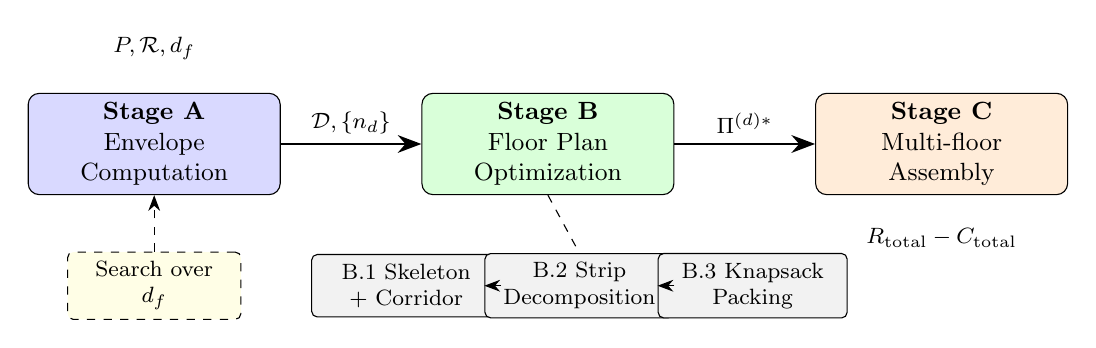
\begin{tikzpicture}[
    stage/.style={draw, rounded corners, minimum width=3.2cm, minimum height=1.1cm, align=center, font=\small},
    substage/.style={draw, rounded corners=2pt, minimum width=2.4cm, minimum height=0.7cm, align=center, font=\footnotesize, fill=gray!10},
    arr/.style={-{Stealth[length=3mm]}, thick},
]
\node[stage, fill=blue!15] (A) at (0,0) {\textbf{Stage A}\\Envelope\\Computation};
\node[stage, fill=green!15] (B) at (5,0) {\textbf{Stage B}\\Floor Plan\\Optimization};
\node[stage, fill=orange!15] (C) at (10,0) {\textbf{Stage C}\\Multi-floor\\Assembly};

\draw[arr] (A) -- (B) node[midway, above, font=\footnotesize] {$\mathcal{D}, \{n_d\}$};
\draw[arr] (B) -- (C) node[midway, above, font=\footnotesize] {$\Pi^{(d)*}$};

\node[above=0.3cm of A, font=\footnotesize, align=center] {$P, \calR, d_f$};

\node[substage] (B1) at (3.2,-1.8) {B.1 Skeleton\\+ Corridor};
\node[substage] (B2) at (5.4,-1.8) {B.2 Strip\\Decomposition};
\node[substage] (B3) at (7.6,-1.8) {B.3 Knapsack\\Packing};

\draw[-{Stealth[length=2mm]}, thin] (B1) -- (B2);
\draw[-{Stealth[length=2mm]}, thin] (B2) -- (B3);
\draw[thin, dashed] (B.south) -- (B2.north);

\node[below=0.3cm of C, font=\footnotesize, align=center] {$R_{\text{total}} - C_{\text{total}}$};

\node[draw, dashed, rounded corners=2pt, minimum width=2.2cm, minimum height=0.7cm, align=center, font=\footnotesize, fill=yellow!10] (df) at (0,-1.8) {Search over\\$d_f$};
\draw[-{Stealth[length=2mm]}, thin, dashed] (df) -- (A.south);
\end{tikzpicture}
\caption{Three-stage decomposition pipeline. Stage~A computes the
buildable envelope for each facade setback candidate $d_f$, producing
the set of distinct footprints $\mathcal{D}$ with floor counts $\{n_d\}$.
Stage~B optimizes the floor plan for each distinct footprint
independently, through skeleton construction, strip decomposition, and
knapsack packing. Stage~C assembles the building and evaluates the
total profit $R_{\text{total}} - C_{\text{total}}$.}
\label{fig:pipeline}
\end{figure}

\begin{remark}[Decomposition Justification]
The decomposition is valid under four structural observations:
\begin{enumerate}[label=(\alph*)]
    \item Once the facade setback distance $d_f$ is fixed, the
    buildable envelope depends only on the lot geometry and regulations,
    not on the apartment layout. No interior design decision can change
    the rasante plane, the shadow cone, or the height limit---these
    are fully determined by $d_f$ and the lot context.
    \item The facade setback $d_f$ is a one-dimensional continuous
    variable that can be efficiently searched by discretization (at
    $\delta$-meter steps) or golden-section search, since the
    total building value as a function of $d_f$ is typically unimodal
    (increasing returns from height eventually overtaken by decreasing
    returns from shrinking footprint).
    \item Floor plans at different levels are coupled only through
    building-wide aggregate constraints (total area, total units,
    structural alignment), not through geometric interactions between
    floors. Once the footprint at each level is known, the interior
    layout of floor~5 does not affect what is feasible on floor~8.
    \item Floors with identical footprints admit identical optimal
    layouts (assuming the same market conditions apply), enabling a
    single floor plan to be replicated across multiple levels. This
    is also consistent with structural engineering practice, where
    column grids are typically maintained vertically for load transfer.
\end{enumerate}
\end{remark}

\begin{example}[Decomposition in Practice]
Consider a trapezoidal corner lot of 2\,000\,m$^2$ in a zone where the
maximum height is a function of the building-to-street distance, with a
constructibility coefficient of 4.5. Stage~A evaluates several facade
setback candidates: at the mandatory minimum setback of 5\,m, the
height regulation allows 8~floors; at 8\,m setback, it allows
11~floors; at 10\,m, it allows the zoning maximum of 12~floors. For
each candidate, the full height map is computed---the rasante from the
narrow street side limits the first 3\,m band to 6~floors, while the
interior reaches the height limit. Stage~A selects the 8\,m setback as
optimal: it produces 3~distinct footprints (floors~1--6 as a large
L-shape, floors~7--9 as a reduced L, floors~10--11 as a compact
rectangle), yielding higher total value than the 5\,m setback (fewer
floors on a larger footprint) or the 10\,m setback (more floors on a
significantly smaller footprint). Stage~B solves three independent
floor plan problems. Stage~C verifies the constructibility constraint
and computes parking for the resulting 58~apartments.
\end{example}


% ═════════════════════════════════════════════════════════════════════════════
\section{Stage A: Buildable Envelope Computation}\label{sec:envelope}
% ═════════════════════════════════════════════════════════════════════════════

The first stage of the optimization determines the three-dimensional
volume within which the building may legally exist. Unlike a naive
approach that would treat this volume as fixed, our formulation
recognizes a critical coupling: the maximum allowable building height
is a function of how far the building facade is set back from the
street. A building placed at the mandatory minimum setback may be
limited to, say, 8~floors; the same building pulled 5 meters further
from the street may be allowed 12~floors. This creates a fundamental
trade-off between \emph{footprint area} (which decreases as the
building retreats from the street) and \emph{building height} (which
increases), and the optimal balance depends on the specific lot
geometry, regulations, and market conditions.

To handle this coupling, we formulate Stage~A as a \emph{parametric
envelope computation}: for each candidate facade setback distance
$d_f$, we compute a complete height map encoding all geometric
regulations, then select the setback that maximizes total building
value. This transforms the coupled 3D geometric problem into a
one-dimensional search over facade positions, each yielding a
self-contained 2D height map.

\subsection{Discretization}

To make the height map computationally tractable, we discretize the lot
polygon onto a regular grid. The choice of resolution $\delta$ balances
accuracy against computation: finer grids capture boundary details more
precisely but increase computation proportionally. A resolution of
$\delta = 0.5$\,m strikes a practical balance, as it is finer than
typical construction tolerances while keeping the grid size manageable
(a 2\,000\,m$^2$ lot produces roughly 8\,000 grid cells).

Let the lot polygon $P$ be embedded in a coordinate system aligned with the
UTM projection (Universal Transverse Mercator, zone~19S for central Chile).
We discretize $P$ into a regular grid:
\[
    G = \bigl\{(i,j) \in \Z^2 : (i\delta, \, j\delta) \in P \bigr\}.
\]

\subsection{Facade Setback as Decision Variable}

Let $\partial P_{\text{street}} = \{\ell_k : k \in K_{\text{street}}\}$
denote the subset of lot boundary segments that face a street, and let
$d_f^{\min}$ be the mandatory minimum front setback (\emph{antejardin}).
The \emph{facade setback distance} $d_f \geq d_f^{\min}$ is the
perpendicular distance from the street-facing boundary to the building
facade line. This distance is a decision variable that determines two
key quantities:

\begin{enumerate}[label=(\roman*)]
    \item \textbf{Maximum building height.} The regulation specifies
    the maximum height as a function of the building-to-street distance:
    \begin{equation}\label{eq:height-vs-setback}
        h_{\max}(d_f) = f(d_f),
    \end{equation}
    where $f$ is a regulatory function (typically piecewise-linear or
    affine). For example, a common formulation is
    $h_{\max}(d_f) = \beta \cdot (d_f + w_{\text{street}})$,
    where $w_{\text{street}}$ is the street width and $\beta$ is a
    coefficient set by the zoning plan (e.g., $\beta = 1.5$ means the
    building height may be up to 1.5 times the distance from the
    building facade to the opposite side of the street). Other zones
    may use step functions, logarithmic formulas, or lookup tables.

    \item \textbf{Buildable footprint area.} Cells between the street
    boundary and the facade line at distance $d_f$ cannot be built upon
    (they form the front garden / setback zone). The set of cells
    available for construction at ground level is:
    \begin{equation}\label{eq:buildable-cells}
        G(d_f) = \bigl\{(i,j) \in G : \text{dist}(i,j;\,\ell_k) \geq d_f,\; \forall k \in K_{\text{street}}\bigr\}.
    \end{equation}
    As $d_f$ increases, $G(d_f)$ shrinks---the building loses frontage
    area.
\end{enumerate}

The trade-off is clear: increasing $d_f$ allows a taller building
(more floors, more total sellable area per unit of footprint) but on a
smaller footprint (fewer apartments per floor). The optimal $d_f$ depends
on the interaction between the height-distance function, the lot depth,
the rasante, and the apartment packing efficiency at different floor
dimensions.

\begin{figure}[ht]
\centering
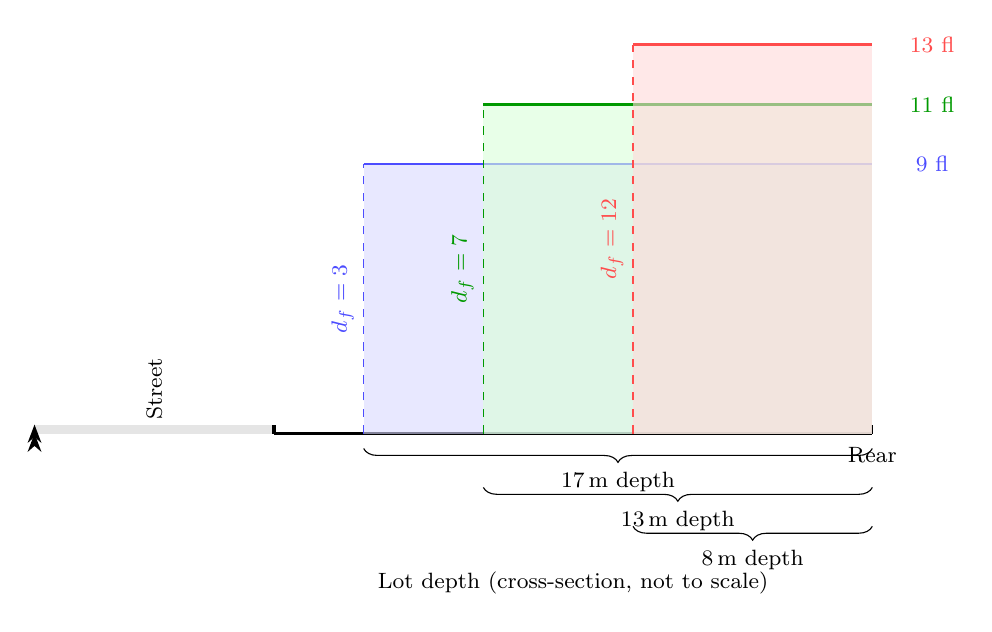
\begin{tikzpicture}[scale=0.38]
\fill[gray!20] (-8,0) rectangle (0,0.3);
\node[font=\footnotesize, rotate=90] at (-4, 1.5) {Street};
\draw[very thick] (0,0) -- (0,0.3);
\draw[thick] (0,0) -- (20,0);
\draw[thick] (20,0) -- (20,0.3);
\node[font=\footnotesize] at (20, -0.7) {Rear};

\fill[blue!15, opacity=0.6] (3,0) rectangle (20, 9);
\draw[dashed, blue!70] (3,0) -- (3,9);
\node[font=\footnotesize, blue!70, rotate=90] at (2.3, 4.5) {$d_f = 3$};
\draw[thick, blue!70] (3, 9) -- (20, 9);
\node[font=\footnotesize, blue!70] at (22, 9) {9 fl};

\fill[green!15, opacity=0.6] (7,0) rectangle (20, 11);
\draw[dashed, green!60!black] (7,0) -- (7,11);
\node[font=\footnotesize, green!60!black, rotate=90] at (6.3, 5.5) {$d_f = 7$};
\draw[thick, green!60!black] (7, 11) -- (20, 11);
\node[font=\footnotesize, green!60!black] at (22, 11) {11 fl};

\fill[red!15, opacity=0.6] (12,0) rectangle (20, 13);
\draw[dashed, red!70] (12,0) -- (12,13);
\node[font=\footnotesize, red!70, rotate=90] at (11.3, 6.5) {$d_f = 12$};
\draw[thick, red!70] (12, 13) -- (20, 13);
\node[font=\footnotesize, red!70] at (22, 13) {13 fl};

\draw[decorate, decoration={brace, amplitude=5pt, mirror}] (3,-0.5) -- (20,-0.5) node[midway, below=5pt, font=\footnotesize] {17\,m depth};
\draw[decorate, decoration={brace, amplitude=5pt, mirror}] (7,-1.8) -- (20,-1.8) node[midway, below=5pt, font=\footnotesize] {13\,m depth};
\draw[decorate, decoration={brace, amplitude=5pt, mirror}] (12,-3.1) -- (20,-3.1) node[midway, below=5pt, font=\footnotesize] {8\,m depth};

\draw[{Stealth}-{Stealth}, thick] (-8, 0) -- (-8, 0.3);
\node[font=\tiny] at (-6, 0.15) {};

\node[font=\footnotesize] at (10, -5) {Lot depth (cross-section, not to scale)};
\end{tikzpicture}
\caption{Facade setback trade-off (cross-section view). Three candidate
setback distances are shown for a 20\,m-deep lot: $d_f = 3$\,m yields
9~floors on 17\,m of depth (blue), $d_f = 7$\,m yields 11~floors on
13\,m (green), and $d_f = 12$\,m yields 13~floors on only 8\,m (red).
The optimal $d_f$ balances height gain against footprint loss.}
\label{fig:setback-tradeoff}
\end{figure}

\subsection{Parametric Height Map}

For a given facade setback $d_f$, we define the height map
$H(\cdot\,; d_f)$ over the buildable cells $G(d_f)$.

\begin{definition}[Parametric Height Map]
The \emph{parametric height map} is a function $H: G(d_f) \times \R_+
\to \N_0$ where $H(i,j;\,d_f)$ represents the maximum number of floors
that can be built at grid cell $(i,j)$ when the building facade is set
back at distance $d_f$ from the street. A cell with $H(i,j;\,d_f) = 0$
lies within a setback zone (lateral or rear) and cannot be built upon
at any height.
\end{definition}

Each regulation $r \in \calR$ imposes an upper bound $H_r(i,j;\,d_f)$
on the buildable height at cell $(i,j)$ under facade setback $d_f$.
Since the building must comply with \emph{all} regulations
simultaneously, the final height map is obtained by taking the
pointwise minimum:
\begin{equation}\label{eq:heightmap}
    H(i,j;\,d_f) = \min_{r \in \calR}\, H_r(i,j;\,d_f), \qquad \forall (i,j) \in G(d_f).
\end{equation}

This formulation preserves the important computational advantage of
independent evaluation: each regulation can be computed independently
(and potentially in parallel), and the results are combined through a
simple elementwise minimum. Adding a new regulation requires only
implementing its height bound function $H_r$; the rest of the pipeline
remains unchanged.

We now define each regulatory constraint formally.

\subsubsection{Maximum Height (Distance-Dependent)}

Unlike a simple zoning cap, the maximum height constraint depends on
the facade setback distance $d_f$. The regulation specifies how tall
the building may be as a function of its distance from the street,
creating the central trade-off of Stage~A.

Let $h_{\max}(d_f)$ be the regulatory maximum building height (in
meters) as given by \eqref{eq:height-vs-setback}, and $h_f$ the
floor-to-floor height (typically 2.7--3.0\,m for residential buildings,
and up to 4.0\,m for the ground floor if commercial use is planned).
The height limit applies uniformly to all cells for a given facade
position:
\begin{equation}
    H_{\text{height}}(i,j;\,d_f) = \left\lfloor \frac{h_{\max}(d_f)}{h_f} \right\rfloor, \qquad \forall (i,j) \in G(d_f).
\end{equation}

Note that while this bound is spatially uniform (all cells share the
same cap for a given $d_f$), it varies across different facade setback
candidates. A setback of $d_f = 5$\,m might yield a cap of 8~floors,
while $d_f = 10$\,m might yield 12~floors.

\begin{example}[Height-Distance Trade-off]
Consider a rectangular lot 20\,m deep (from street to rear boundary)
with mandatory minimum setback $d_f^{\min} = 3$\,m, street width
$w_{\text{street}} = 15$\,m, and $\beta = 1.5$. At $d_f = 3$\,m:
$h_{\max} = 1.5 \times (3 + 15) = 27$\,m $\approx$ 9~floors, with
17\,m of usable depth. At $d_f = 7$\,m: $h_{\max} = 1.5 \times (7 +
15) = 33$\,m $\approx$ 11~floors, but only 13\,m of usable depth. At
$d_f = 12$\,m: $h_{\max} = 1.5 \times (12 + 15) = 40.5$\,m $\approx$
13~floors, but only 8\,m of depth---barely enough for a single
apartment depth plus corridor. The optimal $d_f$ lies somewhere in
this range, balancing height against usable floor area.
\end{example}

\subsubsection{Setbacks (Lateral and Rear)}

Setbacks create mandatory buffer zones between the building and the lot
boundary. The front setback is already captured by the facade setback
variable $d_f$, so the remaining setback constraints apply to the
\emph{lateral} and \emph{rear} boundaries of the lot. These serve
multiple urban planning purposes: lateral separations
(\emph{distanciamiento}) ensure privacy between neighboring buildings,
allow natural ventilation, and provide emergency access corridors; rear
setbacks ensure minimum open space at the back of the lot.

A critical feature of Chilean setback regulations is that lateral
separations \emph{increase with building height}. A 3-story building
might require only a 4\,m lateral separation, while a 10-story building
on the same lot might require 8\,m. This height-dependent setback is
what causes the buildable footprint to shrink at higher floors---the
fundamental mechanism that produces non-rectangular building envelopes.

Let $\{\ell_k\}_{k \in K_{\text{lat}} \cup K_{\text{rear}}}$ denote the
lateral and rear boundary segments (excluding the street-facing segments
already handled by $d_f$). Define the Euclidean distance from a grid
cell to a boundary segment:
\[
    \text{dist}(i,j;\,\ell_k) = \min_{p \in \ell_k} \bigl\|(i\delta,\,j\delta) - p\bigr\|_2.
\]
The setback constraint is:
\begin{equation}
    H_{\text{setback}}(i,j;\,d_f) =
    \begin{cases}
        0 & \text{if } \exists\, k : \text{dist}(i,j;\,\ell_k) < d_k(z) \text{ for } z=1,\\[4pt]
        \max\bigl\{z \in \N : \text{dist}(i,j;\,\ell_k) \geq d_k(z),\ \forall k \in K_{\text{lat}} \cup K_{\text{rear}}\bigr\} & \text{otherwise,}
    \end{cases}
\end{equation}
where $d_k(z)$ is the setback distance at floor $z$. For lateral
separations, this typically follows a linear formula:
$d_k(z) = d_k^{(0)} + \alpha \cdot z \cdot h_f$,
where $d_k^{(0)}$ is the base separation (often 4\,m) and $\alpha$ is
a slope parameter (often derived from the rasante angle). Note that the
lateral setback constraint is independent of $d_f$ (it depends on
distance to lateral/rear boundaries, not to the street), but we write
$H_{\text{setback}}(i,j;\,d_f)$ because the domain $G(d_f)$ changes
with $d_f$.

\subsubsection{Rasante (Inclined Plane)}

The \emph{rasante} is perhaps the most distinctive constraint in Chilean
building regulation. It defines a fixed inclined plane that rises from
each boundary segment at a prescribed angle from the horizontal, and
the building volume must remain entirely below all such planes.
Geometrically, the rasante creates a pyramidal or wedge-shaped envelope:
the building can be tallest at the center of the lot and must taper down
as it approaches any boundary.

The rasante is a \emph{fixed geometric constraint}: the inclined plane
is defined by the lot boundary position and the prescribed angle, and it
does not depend on where the building facade is placed. However, it
interacts with the facade setback indirectly: when the building is
pushed further from the street, the front portion of the lot (between
the street and the facade) is empty, so the rasante from the
street-facing boundary is no longer binding at those cells. The rasante
from lateral and rear boundaries, however, remains fully active.

The rasante angle is set by the zoning plan and typically ranges from
60\textdegree{} to 80\textdegree{} from horizontal. A steeper angle
(closer to 90\textdegree) is more permissive, allowing taller buildings
closer to the boundary; a shallower angle is more restrictive. In many
Chilean zones, the rasante is measured from a point 2--3\,m above the
boundary (the ``base height''), which allows a minimum building height
even at the lot edge.

Let $b_k$ be the base height at segment $\ell_k$ (typically the street
level plus the rasante base offset, often 2--3\,m). The maximum height
at $(i,j)$ due to the rasante from segment $\ell_k$ is:
\begin{equation}
    H_{\text{rasante}}^{(k)}(i,j) = \left\lfloor \frac{b_k + \text{dist}(i,j;\,\ell_k) \cdot \tan(\theta)}{h_f} \right\rfloor.
\end{equation}
The combined rasante constraint is the minimum over all boundary
segments, since the building must lie below the rasante plane from
\emph{every} direction:
\begin{equation}
    H_{\text{rasante}}(i,j;\,d_f) = \min_{k=1,\ldots,K}\, H_{\text{rasante}}^{(k)}(i,j), \qquad \forall (i,j) \in G(d_f).
\end{equation}

Note that $H_{\text{rasante}}^{(k)}$ itself does not depend on $d_f$
(the inclined plane is fixed in space), but its effect on the building
changes because cells in $G(d_f)$ that are far from the street benefit
from a higher rasante allowance at their position. When the building is
set further back, the cells that are actually built upon are further
from the street boundary, where the rasante plane is higher. This is a
second mechanism (beyond the explicit height-distance regulation) by
which increased facade setback allows taller construction.

\begin{example}[Rasante Effect]
Consider a rectangular lot 30\,m deep with rasante angle 70\textdegree{}
and base height 3\,m from the street boundary. With facade setback
$d_f = 5$\,m, the facade line is at 5\,m from the boundary, where the
rasante allows $3 + 5 \cdot \tan(70\textdegree) = 16.7$\,m $\approx$
5~floors. With $d_f = 10$\,m, the facade is at 10\,m, where the
rasante allows $3 + 10 \cdot 2.75 = 30.5$\,m $\approx$ 10~floors. At
the center of the lot (15\,m from the boundary), the rasante allows
$3 + 15 \cdot 2.75 = 44.2$\,m $\approx$ 14~floors regardless of
$d_f$, but this cell is only buildable if $d_f \leq 15$\,m.
\end{example}

\subsubsection{Shadow Projection}

Shadow regulations prevent buildings from casting excessive shadows onto
public spaces during certain hours and seasons. These constraints are
particularly relevant in the southern hemisphere, where the sun tracks
across the northern sky: a tall building on the north side of an
east-west street can cast deep shadows onto the street and neighboring
lots to the south.

The shadow constraint is evaluated at specific solar positions (typically
at solar noon and critical hours during the winter solstice and
equinoxes, as prescribed by the local zoning ordinance). For each
regulated solar position, the shadow cone of a vertical building element
at height $h$ is computed by projecting along the sun vector.

Let $\calS_d$ denote the shadow cone operator for solar direction $d \in
\{$summer, equinox, winter$\}$. For a building element of height $h$ at
position $(x,y)$, the shadow cone projects onto the ground plane as:
\begin{equation}
    \text{Shadow}_d(x,y,h) = \bigl\{(x',y') \in \R^2 : (x',y') = (x,y) + h \cdot \mathbf{v}_d(\tau),\; \tau \in [0,1]\bigr\},
\end{equation}
where $\mathbf{v}_d(\tau)$ is the shadow direction vector at time $\tau$
for season $d$, computed from the solar azimuth and elevation angle at
the lot's latitude. Let $\Omega_{\text{pub}}$ be the set of public spaces
(streets, plazas, parks) whose regulated zones must remain shadow-free
during prescribed hours. The shadow constraint limits the height at each
cell to the tallest value whose shadow does not violate the regulation:
\begin{equation}
    H_{\text{shadow}}(i,j;\,d_f) = \max\bigl\{z \in \N : \text{Shadow}_d\bigl(i\delta,\,j\delta,\,z \cdot h_f\bigr) \cap \Omega_{\text{pub}} = \emptyset,\; \forall d\bigr\}.
\end{equation}

The shadow constraint also interacts with the facade setback: when the
building is set further back, its shadow-casting facade is further from
the street, so the shadow must travel a longer distance before reaching
the regulated public space. This allows taller construction at the
facade line. Conversely, for cells deep inside the lot (far from the
street), the shadow constraint is typically non-binding because their
shadows fall onto the lot itself.

\subsection{Optimal Facade Setback Selection}\label{sec:facade-opt}

The central optimization in Stage~A is the selection of the facade
setback distance $d_f^*$ that maximizes the total building value. For
each candidate setback, the parametric height map $H(\cdot\,;\,d_f)$
yields a set of floor footprints, which in turn determine the floor
plan values (computed in Stages~B and~C). The optimization is:
\begin{equation}\label{eq:facade-opt}
    d_f^* = \argmax_{d_f \in \{d_f^{\min},\, d_f^{\min} + \delta,\, \ldots,\, d_f^{\max}\}} \; \text{BuildingValue}\bigl(H(\cdot\,;\,d_f)\bigr),
\end{equation}
where $d_f^{\max}$ is a practical upper bound on the setback (beyond
which the remaining footprint is too small for a viable building), and
$\text{BuildingValue}(\cdot)$ is the total profit from Stages~B and~C
evaluated on the height map.

The search space is small: with $\delta = 0.5$\,m resolution and a
typical range of 3--15\,m, there are at most 25 candidate values. For
each candidate, the height map computation is $O(|G| \cdot |\calR|
\cdot K)$, and the subsequent floor plan optimization (Stages~B and~C)
is sub-millisecond. The entire facade optimization therefore completes
in well under one second.

\begin{remark}[Unimodality]
In practice, the total building value as a function of $d_f$ is
typically unimodal: it increases as additional floors more than
compensate for lost footprint area, reaches a peak, and then decreases
as the footprint becomes too narrow for efficient apartment packing.
This unimodality allows the use of golden-section search instead of
exhaustive enumeration, reducing the number of evaluations to
$O(\log(1/\delta))$. However, given the small search space, exhaustive
evaluation at every $\delta$-step is equally practical and avoids
assumptions about the value function shape.
\end{remark}

\subsection{Floor Footprint Extraction}

Once the optimal facade setback $d_f^*$ is selected, the height map
$H(\cdot) \equiv H(\cdot\,;\,d_f^*)$ is fixed, and the floor footprints
are extracted. The footprint at floor level $z$ consists of all
buildable cells where the height map meets or exceeds $z$:
\begin{equation}\label{eq:footprint}
    \calF_z = \bigl\{(i,j) \in G(d_f^*) : H(i,j;\,d_f^*) \geq z\bigr\}, \qquad z = 1, \ldots, Z_{\max},
\end{equation}
where $Z_{\max} = \max_{(i,j) \in G(d_f^*)} H(i,j;\,d_f^*)$ is the
maximum building height anywhere on the lot under the chosen setback.

By construction, the footprints form a nested (monotone decreasing)
sequence:
\[
    \calF_1 \supseteq \calF_2 \supseteq \cdots \supseteq \calF_{Z_{\max}}.
\]

\begin{figure}[ht]
\centering
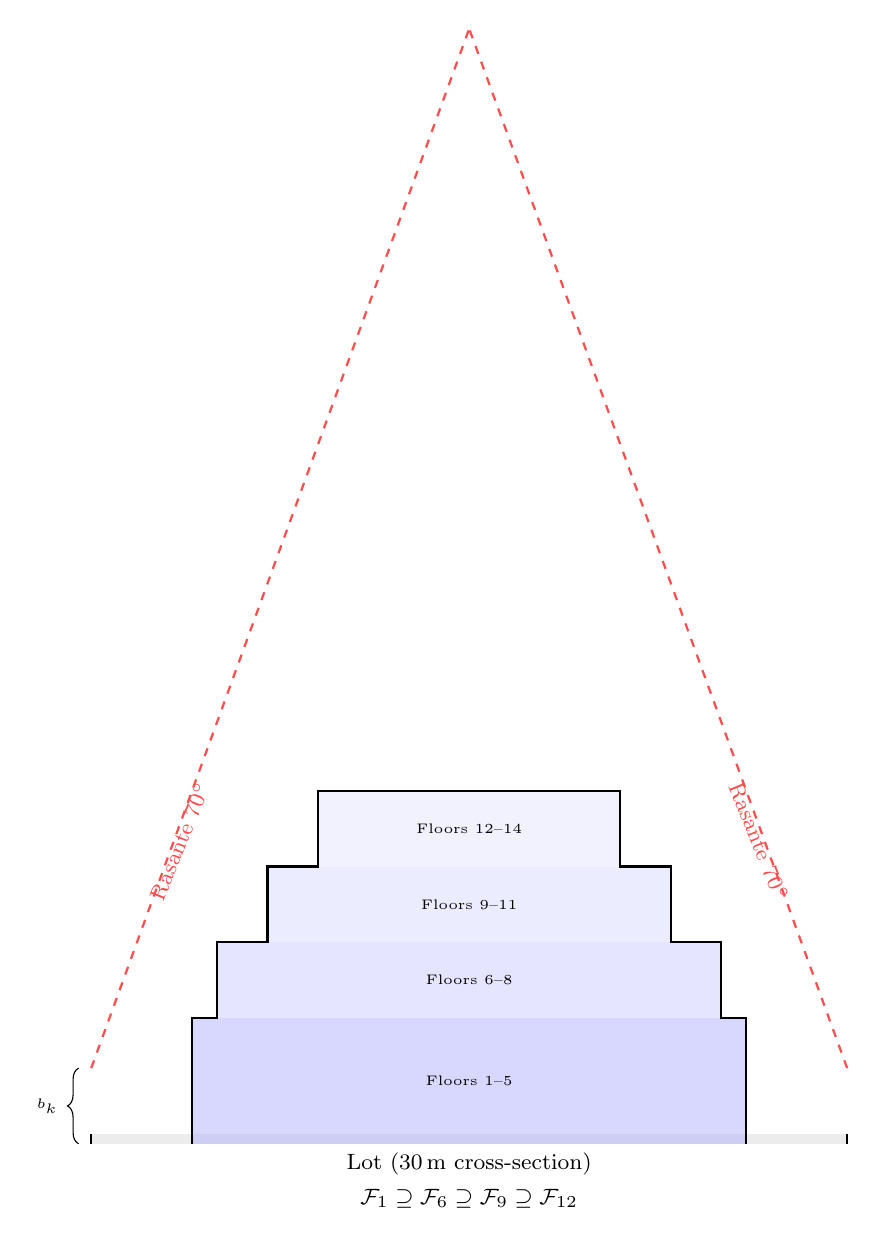
\begin{tikzpicture}[scale=0.32]
\fill[gray!15] (0,0) rectangle (30, 0.4);
\node[font=\footnotesize] at (15, -0.8) {Lot (30\,m cross-section)};

\draw[thick, red!70, dashed] (0,3) -- (15, 3+15*2.75);
\draw[thick, red!70, dashed] (30,3) -- (15, 3+15*2.75);
\node[font=\footnotesize, red!70, rotate=68] at (3.5, 12) {Rasante $70^\circ$};
\node[font=\footnotesize, red!70, rotate=-68] at (26.5, 12) {Rasante $70^\circ$};

\fill[blue!30, opacity=0.5] (4,0) rectangle (26, 5);
\fill[blue!20, opacity=0.5] (5,5) rectangle (25, 8);
\fill[blue!15, opacity=0.5] (7,8) rectangle (23, 11);
\fill[blue!10, opacity=0.5] (9,11) rectangle (21, 14);

\draw[thick] (4,0) -- (4,5) -- (5,5) -- (5,8) -- (7,8) -- (7,11) -- (9,11) -- (9,14) -- (21,14) -- (21,11) -- (23,11) -- (23,8) -- (25,8) -- (25,5) -- (26,5) -- (26,0);

\node[font=\tiny] at (15, 2.5) {Floors 1--5};
\node[font=\tiny] at (15, 6.5) {Floors 6--8};
\node[font=\tiny] at (15, 9.5) {Floors 9--11};
\node[font=\tiny] at (15, 12.5) {Floors 12--14};

\draw[decorate, decoration={brace, amplitude=4pt}] (-0.5,0) -- (-0.5,3) node[midway, left=4pt, font=\tiny] {$b_k$};

\draw[thick] (0,0) -- (0,0.4);
\draw[thick] (30,0) -- (30,0.4);

\node[font=\footnotesize] at (15, -2.2) {$\calF_1 \supseteq \calF_6 \supseteq \calF_9 \supseteq \calF_{12}$};
\end{tikzpicture}
\caption{Building cross-section shaped by the rasante constraint
(not to scale). The rasante planes from both lateral boundaries create
a tapered envelope. The building steps back at higher floors, producing
nested footprints $\calF_1 \supseteq \calF_6 \supseteq \calF_9
\supseteq \calF_{12}$. Each distinct footprint defines a group of
floors with identical plans.}
\label{fig:rasante-envelope}
\end{figure}

Lower floors have larger footprints because the lateral setback and
rasante constraints are less restrictive close to ground level; upper
floors have progressively smaller footprints as the inclined planes and
height-dependent separations take effect. The front boundary of every
footprint is at distance $d_f^*$ from the street (the facade line),
while the lateral and rear boundaries recede inward at higher floors.

We define the set of \emph{distinct footprints}---footprints that define
genuinely different polygons---since consecutive floors often share the
same footprint (e.g., floors 3 through 7 might all have identical
outlines because no regulation changes in that height range):
\begin{equation}
    \mathcal{D} = \bigl\{\calF_z : z \in \{1,\ldots,Z_{\max}\}\bigr\} \big/ {\sim},
\end{equation}
where $\calF_z \sim \calF_{z'}$ if they define the same polygon. Let
$|\mathcal{D}|$ denote the number of distinct footprints. For each
$\calF \in \mathcal{D}$, let $n(\calF)$ be the number of floors sharing
that footprint.

In practice, $|\mathcal{D}|$ is small---typically 2 to 5 for buildings
up to 15 floors. This is because the regulations change in discrete
steps (a floor either fits within the rasante or it doesn't), so the
footprint changes only at a few critical heights.

\subsection{Ground Occupation Constraint}

The ground occupation coefficient limits how much of the lot can be
covered by the building at ground level. This constraint ensures
permeable surfaces, green areas, and pedestrian circulation at grade.

Let $c_{\text{occ}}$ be the maximum ground occupation coefficient. The
ground floor footprint must satisfy:
\begin{equation}
    \text{Area}(\calF_1) \leq c_{\text{occ}} \cdot \text{Area}(P).
\end{equation}
If this constraint is violated (which can occur when the facade setback
$d_f^*$ produces a large ground-level footprint), cells in $\calF_1$ are
removed starting from the interior cells furthest from the corridor axis
(preserving connectivity and compactness) until the constraint is
satisfied. This may also constrain the facade setback search: candidates
$d_f$ for which even the reduced $\calF_1$ is architecturally
impractical are discarded.


% ═════════════════════════════════════════════════════════════════════════════
\section{Stage B: Floor Plan Optimization}\label{sec:floorplan}
% ═════════════════════════════════════════════════════════════════════════════

With the buildable envelope computed, the next stage addresses the core
combinatorial challenge: determining the optimal internal layout of each
floor. In a corridor-based residential building---the dominant typology
for mid-rise urban development---each floor consists of a central
corridor providing access to apartments arranged on both sides, a
circulation core (staircase and elevator shaft), and possibly terraces
or common areas at the ends.

The key geometric observation is that apartments in these buildings are
arranged in a \emph{linear sequence} along the corridor. Each apartment
occupies a rectangular slot defined by its \emph{frontage width}
(parallel to the corridor) and \emph{depth} (perpendicular to the
corridor, extending to the facade). This linear arrangement means that
once the corridor position and orientation are fixed, the problem of
assigning apartments to each side of the corridor reduces to a
\emph{one-dimensional packing problem}---specifically, a bounded
knapsack.

However, real floor footprints are not always rectangular. The
height-dependent setbacks from Stage~A commonly produce L-shaped,
U-shaped, H-shaped, or T-shaped footprints, especially at lower floors
of corner lots or lots with irregular boundaries. A corridor in an
L-shaped floor must turn a corner; an H-shaped floor may require a
branching corridor. The medial axis of the floor polygon provides a
natural and mathematically principled way to determine where the corridor
should run.

For each distinct footprint $\calF \in \mathcal{D}$, we optimize the floor
plan independently. The optimization proceeds in four sub-stages.


% ─────────────────────────────────────────────────────────────────────────────
\subsection{Stage B.1: Skeleton Graph and Corridor Routing}\label{sec:skeleton}
% ─────────────────────────────────────────────────────────────────────────────

\subsubsection{Rectilinear Medial Axis}

The first step is to determine where the corridor should run within the
floor footprint. Intuitively, the corridor should pass through the
``center'' of the polygon so that apartments on both sides have
approximately equal and maximal depth. The mathematical tool for this
is the \emph{medial axis}---the set of points inside the polygon that
are equidistant from at least two boundary edges. For a rectangular
footprint, the medial axis is simply the centerline; for an L-shaped
footprint, it is an L-shaped line running through the center of each
arm.

Let $\calF$ be a rectilinear polygon (which it will be, since the grid
discretization produces axis-aligned boundaries). Its \emph{medial axis}
$M(\calF)$ is the locus of points equidistant from the two nearest
boundary edges. For rectilinear polygons, $M(\calF)$ is a rectilinear
tree---a tree graph where all segments are axis-aligned (horizontal or
vertical).

\begin{definition}[Skeleton Graph]
The \emph{skeleton graph} $\calG = (V, E)$ is a graph derived from the
medial axis by snapping its vertices to a structural grid:
\begin{itemize}[nosep]
    \item $V$ is the set of vertices of $M(\calF)$ snapped to the
    structural grid $\Gamma = \{(x,y) : x \in \Gamma_x,\, y \in
    \Gamma_y\}$, where $\Gamma_x$ and $\Gamma_y$ are the column and
    beam positions (typically spaced 6--8\,m apart, reflecting
    standard reinforced-concrete structural spans),
    \item $E$ is the set of axis-aligned segments connecting adjacent
    vertices along $M(\calF)$.
\end{itemize}
\end{definition}

The snapping to a structural grid is architecturally motivated: in
reinforced-concrete construction (the dominant method for mid-rise
residential buildings), columns must be arranged on a regular grid for
efficient load transfer. The corridor axis naturally aligns with one
direction of this grid, and apartment partition walls align with the
other.

In practice, $|V| \leq 6$ and $|E| \leq 8$ for the floor shapes
encountered in urban development (L, H, U, T, and rectangular). This
small size is a consequence of the fact that urban lots, while
irregular, produce floor footprints that are compositions of a small
number of rectangular blocks.

\begin{figure}[ht]
\centering
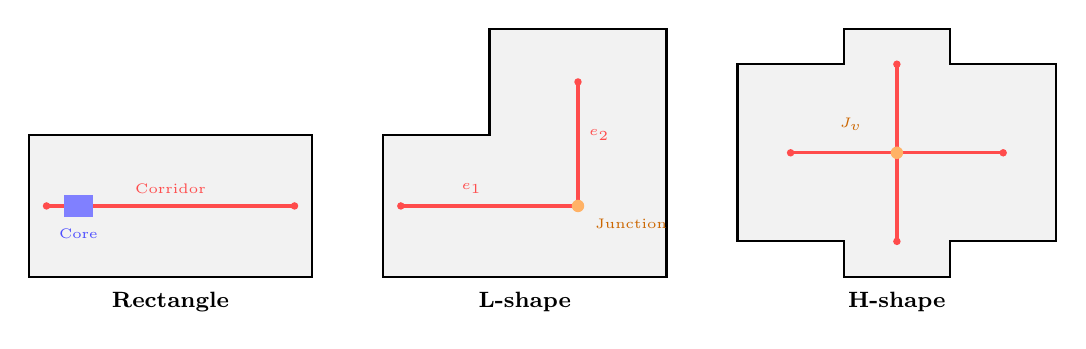
\begin{tikzpicture}[scale=0.45]
\begin{scope}[shift={(0,0)}]
    \fill[gray!10] (0,0) rectangle (8,4);
    \draw[thick] (0,0) rectangle (8,4);
    \draw[very thick, red!70] (0.5,2) -- (7.5,2);
    \fill[red!70] (0.5,2) circle (3pt);
    \fill[red!70] (7.5,2) circle (3pt);
    \node[font=\footnotesize\bfseries] at (4, -0.7) {Rectangle};
    \node[font=\tiny, red!70] at (4, 2.5) {Corridor};
    \fill[blue!50] (1, 1.7) rectangle (1.8, 2.3);
    \node[font=\tiny, blue!70] at (1.4, 1.2) {Core};
\end{scope}

\begin{scope}[shift={(10,0)}]
    \fill[gray!10] (0,0) rectangle (8,4);
    \fill[gray!10] (3,4) rectangle (8,7);
    \draw[thick] (0,0) -- (8,0) -- (8,7) -- (3,7) -- (3,4) -- (0,4) -- cycle;
    \draw[very thick, red!70] (0.5,2) -- (5.5,2) -- (5.5,5.5);
    \fill[red!70] (0.5,2) circle (3pt);
    \fill[red!70] (5.5,2) circle (3pt);
    \fill[red!70] (5.5,5.5) circle (3pt);
    \node[font=\footnotesize\bfseries] at (4, -0.7) {L-shape};
    \node[font=\tiny, red!70] at (2.5, 2.5) {$e_1$};
    \node[font=\tiny, red!70] at (6.1, 4) {$e_2$};
    \fill[orange!60] (5.5,2) circle (5pt);
    \node[font=\tiny, orange!80!black] at (7, 1.5) {Junction};
\end{scope}

\begin{scope}[shift={(20,0)}]
    \fill[gray!10] (0,1) rectangle (3,6);
    \fill[gray!10] (3,0) rectangle (6,7);
    \fill[gray!10] (6,1) rectangle (9,6);
    \draw[thick] (0,1) -- (0,6) -- (3,6) -- (3,7) -- (6,7) -- (6,6) -- (9,6) -- (9,1) -- (6,1) -- (6,0) -- (3,0) -- (3,1) -- cycle;
    \draw[very thick, red!70] (1.5,3.5) -- (4.5,3.5) -- (7.5,3.5);
    \draw[very thick, red!70] (4.5,1) -- (4.5,6);
    \fill[red!70] (1.5,3.5) circle (3pt);
    \fill[red!70] (7.5,3.5) circle (3pt);
    \fill[red!70] (4.5,1) circle (3pt);
    \fill[red!70] (4.5,6) circle (3pt);
    \fill[orange!60] (4.5,3.5) circle (5pt);
    \node[font=\footnotesize\bfseries] at (4.5, -0.7) {H-shape};
    \node[font=\tiny, orange!80!black] at (3.2, 4.3) {$J_v$};
\end{scope}
\end{tikzpicture}
\caption{Skeleton graphs (red) for three common floor plan shapes.
Vertices (dots) mark corridor endpoints and junctions; edges define
corridor segments. The \textbf{rectangle} has a single straight
corridor. The \textbf{L-shape} has a two-edge corridor with one
junction (orange) at the corner. The \textbf{H-shape} has a
cross-shaped corridor with a central junction. The blue square marks
a possible circulation core placement.}
\label{fig:skeleton-topologies}
\end{figure}

\subsubsection{Corridor as Connected Subtree}

A \emph{corridor} is a connected subtree $\calC \subseteq \calG$ with
uniform width $w_c$ (typically 1.5--2.0\,m, set by building code
requirements for emergency egress). The corridor polygon is obtained by
buffering the subtree by half the corridor width:
\[
    P_{\calC} = \bigl\{p \in \R^2 : \text{dist}(p, \calC) \leq w_c/2\bigr\}.
\]

Not every connected subtree of $\calG$ constitutes a usable corridor.
A valid corridor must reach all parts of the floor footprint (so that
every apartment has access) and must accommodate the circulation core
(staircase and elevator) at one of its vertices.

\begin{definition}[Valid Corridor]
A corridor $\calC$ is \emph{valid} if:
\begin{enumerate}[label=(\roman*)]
    \item \textbf{Coverage:} Every point in the floor footprint is within
    a maximum access distance $d_{\text{acc}}$ from the corridor:
    \begin{equation}\label{eq:corridor-valid}
        \max_{p \in \calF} \text{dist}(p, P_{\calC}) \leq d_{\text{acc}}.
    \end{equation}
    This ensures that no apartment is located unreasonably far from the
    corridor, as required by fire safety codes and practical livability.
    \item \textbf{Circulation core placement:} $\calC$ must contain at
    least one vertex $v \in V$ where a circulation core of dimensions
    $w_{\text{core}} \times d_{\text{core}}$ (typically 6\,m $\times$
    5\,m, accommodating one elevator and one fire staircase) can be
    placed without overlapping the lot boundary.
\end{enumerate}
\end{definition}

Let $\calC^* = \{\calC_1, \ldots, \calC_M\}$ be the set of all valid
corridors. Since $\calG$ is small, the enumeration of all connected
subtrees is computationally trivial: $|\calC^*|$ is typically 2--10.

\begin{example}[Corridor Topologies]
For a \textbf{rectangular} footprint, there is typically one corridor
option: a single straight segment running the length of the rectangle.
For an \textbf{L-shaped} footprint, there are typically 2--3 options:
(a)~an L-shaped corridor following both arms, (b)~a corridor running
along only the longer arm, and (c)~a corridor running along only the
shorter arm. Option~(a) serves the entire floor but introduces a
junction (corner); options~(b) and~(c) leave part of the floor
unserved but avoid the junction. For an \textbf{H-shaped} footprint,
the corridor typically has a T or cross configuration, with junctions
at each branching point.
\end{example}


% ─────────────────────────────────────────────────────────────────────────────
\subsection{Stage B.2: Strip Decomposition}\label{sec:strips}
% ─────────────────────────────────────────────────────────────────────────────

Once a corridor is chosen, the usable floor area naturally divides into
rectangular \emph{strips}---the bands of space on each side of each
corridor segment where apartments can be placed. This decomposition is
the crucial step that reduces the two-dimensional floor plan layout
to a collection of independent one-dimensional packing problems.

\subsubsection{Strip Segments}

Given a valid corridor $\calC_m \in \calC^*$, the usable floor area
(everything that is not corridor, circulation core, or structural
elements) is:
\[
    U_m = \calF \setminus P_{\calC_m}.
\]

Each edge $e \in E(\calC_m)$ is an axis-aligned segment. For a horizontal
edge $e$ at ordinate $y_e$ spanning the interval $[x_e^L, x_e^R]$, the
corridor creates two strips---one on the north side and one on the south
side:
\begin{align}
    S_e^{+} &= U_m \cap \bigl\{(x,y) : x \in [x_e^L, x_e^R],\ y \in [y_e + w_c/2,\ y_e + w_c/2 + D_{\max}]\bigr\}, \label{eq:strip-north} \\
    S_e^{-} &= U_m \cap \bigl\{(x,y) : x \in [x_e^L, x_e^R],\ y \in [y_e - w_c/2 - D_{\max},\ y_e - w_c/2]\bigr\}, \label{eq:strip-south}
\end{align}
where $D_{\max}$ is the maximum apartment depth (interior depth plus
terrace, typically 12--16\,m, bounded by natural light penetration
requirements). Vertical edges produce analogous east/west strips.

The intersection with $U_m$ in the definitions above is important: it
clips the strips to the actual footprint boundary, so that a strip along
a corridor edge near the lot boundary may be shallower than $D_{\max}$.

\begin{figure}[ht]
\centering
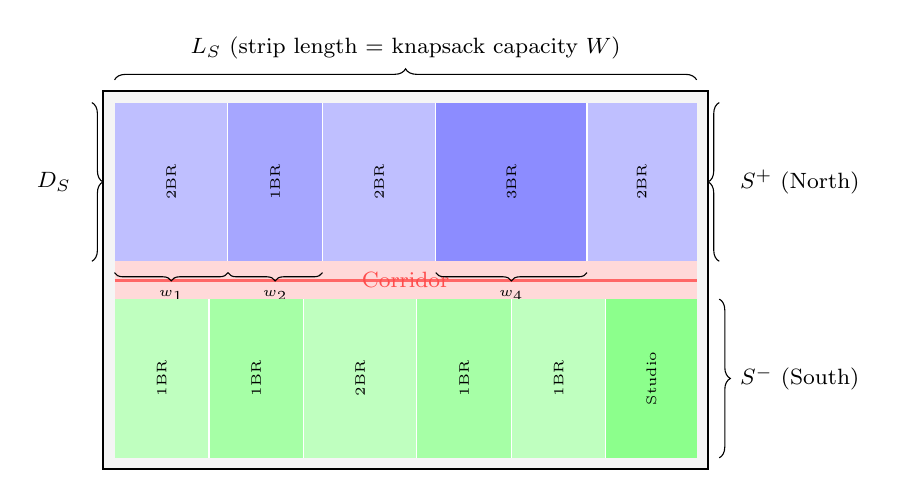
\begin{tikzpicture}[scale=0.48]
\fill[gray!8] (0,0) rectangle (16,10);
\draw[thick] (0,0) rectangle (16,10);

\fill[red!15] (0.3, 4.5) rectangle (15.7, 5.5);
\draw[very thick, red!60] (0.3, 5) -- (15.7, 5);
\node[font=\footnotesize, red!70] at (8, 5) {Corridor};

\fill[blue!10] (0.3, 5.5) rectangle (15.7, 9.7);
\fill[green!10] (0.3, 0.3) rectangle (15.7, 4.5);

\draw[decorate, decoration={brace, amplitude=4pt}] (16.3, 5.5) -- (16.3, 9.7) node[midway, right=4pt, font=\footnotesize] {$S^+$ (North)};
\draw[decorate, decoration={brace, amplitude=4pt, mirror}] (16.3, 0.3) -- (16.3, 4.5) node[midway, right=4pt, font=\footnotesize] {$S^-$ (South)};

\draw[decorate, decoration={brace, amplitude=4pt}] (0.3, 10.3) -- (15.7, 10.3) node[midway, above=4pt, font=\footnotesize] {$L_S$ (strip length = knapsack capacity $W$)};

\fill[blue!25] (0.3, 5.5) rectangle (3.3, 9.7);
\fill[blue!35] (3.3, 5.5) rectangle (5.8, 9.7);
\fill[blue!25] (5.8, 5.5) rectangle (8.8, 9.7);
\fill[blue!45] (8.8, 5.5) rectangle (12.8, 9.7);
\fill[blue!25] (12.8, 5.5) rectangle (15.7, 9.7);
\draw[thin, white] (3.3, 5.5) -- (3.3, 9.7);
\draw[thin, white] (5.8, 5.5) -- (5.8, 9.7);
\draw[thin, white] (8.8, 5.5) -- (8.8, 9.7);
\draw[thin, white] (12.8, 5.5) -- (12.8, 9.7);

\node[font=\tiny, rotate=90] at (1.8, 7.6) {2BR};
\node[font=\tiny, rotate=90] at (4.55, 7.6) {1BR};
\node[font=\tiny, rotate=90] at (7.3, 7.6) {2BR};
\node[font=\tiny, rotate=90] at (10.8, 7.6) {3BR};
\node[font=\tiny, rotate=90] at (14.25, 7.6) {2BR};

\draw[decorate, decoration={brace, amplitude=3pt, mirror}] (0.3, 5.2) -- (3.3, 5.2) node[midway, below=3pt, font=\tiny] {$w_1$};
\draw[decorate, decoration={brace, amplitude=3pt, mirror}] (3.3, 5.2) -- (5.8, 5.2) node[midway, below=3pt, font=\tiny] {$w_2$};
\draw[decorate, decoration={brace, amplitude=3pt, mirror}] (8.8, 5.2) -- (12.8, 5.2) node[midway, below=3pt, font=\tiny] {$w_4$};

\fill[green!25] (0.3, 0.3) rectangle (2.8, 4.5);
\fill[green!35] (2.8, 0.3) rectangle (5.3, 4.5);
\fill[green!25] (5.3, 0.3) rectangle (8.3, 4.5);
\fill[green!35] (8.3, 0.3) rectangle (10.8, 4.5);
\fill[green!25] (10.8, 0.3) rectangle (13.3, 4.5);
\fill[green!45] (13.3, 0.3) rectangle (15.7, 4.5);
\draw[thin, white] (2.8, 0.3) -- (2.8, 4.5);
\draw[thin, white] (5.3, 0.3) -- (5.3, 4.5);
\draw[thin, white] (8.3, 0.3) -- (8.3, 4.5);
\draw[thin, white] (10.8, 0.3) -- (10.8, 4.5);
\draw[thin, white] (13.3, 0.3) -- (13.3, 4.5);

\node[font=\tiny, rotate=90] at (1.55, 2.4) {1BR};
\node[font=\tiny, rotate=90] at (4.05, 2.4) {1BR};
\node[font=\tiny, rotate=90] at (6.8, 2.4) {2BR};
\node[font=\tiny, rotate=90] at (9.55, 2.4) {1BR};
\node[font=\tiny, rotate=90] at (12.05, 2.4) {1BR};
\node[font=\tiny, rotate=90] at (14.5, 2.4) {Studio};

\draw[decorate, decoration={brace, amplitude=4pt, mirror}] (-0.3, 5.5) -- (-0.3, 9.7) node[midway, left=4pt, font=\footnotesize] {$D_S$};
\end{tikzpicture}
\caption{Strip decomposition of a rectangular floor plan. The corridor
(red) divides the floor into two strips: $S^+$ (north-facing) and $S^-$
(south-facing). Each strip is packed independently with apartment
templates via the bounded knapsack: template widths $w_t$ consume strip
length $L_S$, while template depths must fit within strip depth $D_S$.
Different shading intensities indicate different apartment types.}
\label{fig:strip-packing}
\end{figure}

Each strip $S$ is characterized by three key parameters:
\begin{itemize}[nosep]
    \item \textbf{Length $L_S$}: the dimension parallel to the corridor
    edge. This determines how many apartments can fit side by side---it
    is the ``capacity'' of the knapsack.
    \item \textbf{Depth $D_S$}: the dimension perpendicular to the
    corridor (available for apartment depth + terrace). This determines
    which apartment templates are feasible---only templates whose total
    depth (interior + terrace) fits within $D_S$ can be placed.
    \item \textbf{Orientation $\theta_S \in \{$N, S, E, W, NE, NW, SE,
    SW$\}$}: the outward-facing direction of the strip, determined by
    which side of the corridor the strip lies on and the compass
    bearing of the lot boundary. Orientation affects apartment revenue
    through market preferences (north-facing apartments command premium
    prices in the southern hemisphere due to superior solar exposure).
\end{itemize}

Strips with $L_S < w_{\min}^{\text{apt}}$ (minimum apartment width,
typically 5--6\,m) or $D_S < d_{\min}^{\text{apt}}$ (minimum apartment
depth, typically 4--5\,m) are discarded as too small to accommodate any
apartment template.

\subsubsection{Junction Zones}

Where the corridor changes direction---at each vertex of the corridor
subtree with degree $\geq 2$---a \emph{junction zone} arises. These
are the irregular regions at corridor intersections where the simple
strip model does not directly apply. The design treatment of each
junction significantly affects the overall floor plan quality and must
be handled explicitly.

A \emph{junction} occurs at each vertex $v \in V(\calC_m)$ with degree
$\geq 2$. The junction zone $J_v$ is the rectangular region at the
corridor intersection:
\begin{equation}
    J_v = \bigl\{(x,y) : |x - x_v| \leq r_J,\ |y - y_v| \leq r_J\bigr\} \cap \calF,
\end{equation}
where $r_J$ is the junction radius (typically half the structural grid
spacing, i.e., 3--4\,m). Let $\calJ_m = \{J_1, \ldots, J_{|\calJ_m|}\}$
be the set of junctions for corridor $\calC_m$.

Each junction $J_v$ admits a discrete set of \emph{junction options}
$\calO_v$, representing the different architectural treatments of the
junction zone:
\begin{enumerate}[label=(\alph*)]
    \item \textbf{Circulation core}: Place the staircase and elevator
    shaft at the junction. This is often the architecturally natural
    location for the core, as it provides equal access to all corridor
    branches. However, it consumes area from adjacent strips (reducing
    their usable length) and generates no direct revenue.
    Revenue contribution: $0$.

    \item \textbf{Corner apartment}: An L-shaped apartment that wraps
    around the corridor turn, with frontage on two perpendicular
    corridor edges. These units are architecturally desirable because
    they have dual exposure (windows facing two directions), commanding
    a market premium. However, they require sufficient depth in both
    adjacent strips and introduce a non-rectangular floor plan for that
    unit. Revenue contribution: $r_{\text{corner}}$ (premium for dual
    exposure, typically 5--15\% above a standard unit of the same area).

    \item \textbf{Common area}: Leave the junction as lobby space, a
    small lounge, or an amenity area (mailroom, bicycle parking access).
    This does not consume strip length or generate revenue, but may be
    required for building code compliance (e.g., a minimum lobby area
    per floor) or market positioning.
    Revenue contribution: $0$, but no strip area consumed either.
\end{enumerate}

Each option $o \in \calO_v$ reduces the available length of adjacent
strips by a known amount $\Delta L_{v,s}^{(o)}$ for each adjacent strip
$s$. For instance, placing a circulation core of width 6\,m at a junction
reduces the length of each adjacent strip by 3\,m (half the core, as
the other half extends into the opposite strip).


% ─────────────────────────────────────────────────────────────────────────────
\subsection{Stage B.3: Apartment Template Packing}\label{sec:knapsack}
% ─────────────────────────────────────────────────────────────────────────────

With the floor decomposed into strips of known length, depth, and
orientation, the problem of placing apartments on each strip becomes a
classical one-dimensional bounded knapsack problem. This is the
computational heart of the floor plan optimization: it determines which
apartments go where, and directly produces the economic value of each
floor.

\subsubsection{Apartment Templates}

Unlike the current approach of generating apartments as generic
rectangles and assigning types \emph{after} optimization, our formulation
defines apartment templates \emph{from} market-driven type specifications.
Each template represents a specific architectural configuration with
known dimensions, area, and market value.

\begin{definition}[Apartment Template]
An \emph{apartment template} is a tuple $t = (\tau, w_t, d_t, d_t^{\text{ter}}, a_t, a_t^{\text{ter}}, r_t)$ where:
\begin{itemize}[nosep]
    \item $\tau \in \calT$ is the apartment type (e.g., studio, 1BR,
    2BR, 3BR), each with specific architectural requirements (number
    of bedrooms, bathrooms, minimum kitchen area),
    \item $w_t$ is the \emph{frontage width} (parallel to corridor),
    constrained by bedroom layout: a studio may need only 5\,m of
    frontage, while a 3BR apartment typically needs 9--12\,m to
    accommodate three bedrooms side by side,
    \item $d_t$ is the \emph{interior depth} (perpendicular to corridor),
    bounded above by natural light requirements: a depth of 12--14\,m is
    the practical maximum for single-exposure residential units, as
    interior spaces beyond this distance receive insufficient daylight,
    \item $d_t^{\text{ter}}$ is the terrace depth,
    \item $a_t = w_t \cdot d_t$ is the interior area,
    \item $a_t^{\text{ter}} = w_t \cdot d_t^{\text{ter}}$ is the terrace area,
    \item $r_t$ is the total revenue, computed from market prices per
    usable square meter.
\end{itemize}
\end{definition}

The set of all templates is denoted $\calT_{\text{all}}$. For a strip $S$
with depth $D_S$, the \emph{feasible templates} are those whose total
depth (interior + terrace) fits within the available strip depth:
\begin{equation}
    \calT_S = \bigl\{t \in \calT_{\text{all}} : d_t + d_t^{\text{ter}} \leq D_S\bigr\}.
\end{equation}

Templates are generated from market data: for each apartment type
$\tau \in \calT$, the width and depth ranges are bounded by
architectural constraints that reflect real design practice:
\begin{equation}
    w_\tau^{\min} \leq w_t \leq w_\tau^{\max}, \qquad
    d_\tau^{\min} \leq d_t \leq d_\tau^{\max}, \qquad
    a_\tau^{\min} \leq a_t \leq a_\tau^{\max}.
\end{equation}

For example, a 2BR apartment might have $w \in [7, 10]$\,m, $d \in [7,
12]$\,m, and $a \in [50, 75]$\,m$^2$. The discrete template set is
generated by sampling these ranges at a resolution of $\delta_w = 0.5$\,m
and filtering to keep only architecturally valid configurations (e.g.,
aspect ratios between 0.5 and 2.0, area within type-specific bounds).

The terrace depth is determined by interpolation from market-typical
terrace areas:
\begin{equation}
    d_t^{\text{ter}} = \text{clamp}\!\left(\frac{A_{\text{ter}}(a_t)}{w_t},\; d_{\text{ter}}^{\min},\; d_{\text{ter}}^{\max}\right),
\end{equation}
where $A_{\text{ter}}(\cdot)$ is a piecewise-linear interpolation of
typical terrace areas by interior area, derived from market transaction
data. Smaller apartments tend to have proportionally smaller terraces;
larger units may have terraces of 10--20\,m$^2$.

The revenue per template incorporates an orientation quality factor that
reflects market preferences for solar exposure:
\begin{equation}\label{eq:revenue}
    r_t(\theta_S) = \bigl(a_t + 0.5\, a_t^{\text{ter}}\bigr) \cdot p_\tau \cdot \phi(\theta_S),
\end{equation}
where $p_\tau$ is the price per usable square meter for type $\tau$
(derived from comparable market transactions), and $\phi(\theta_S) \in
(0,1]$ is an orientation quality factor. In the Chilean market, the
factor $0.5$ on terrace area reflects the convention that terraces
contribute half their area to the ``usable surface'' for pricing
purposes (matching the legal definition in Chilean real estate law).
Typical orientation factors are $\phi(\text{N}) = 1.0$ (full northern
sun), $\phi(\text{NE}) = \phi(\text{NW}) = 0.95$, $\phi(\text{E}) =
\phi(\text{W}) = 0.90$, $\phi(\text{S}) = 0.85$ (least desirable in
the southern hemisphere).

\subsubsection{Bounded Knapsack Formulation}

For a single strip $S$ with length $L_S$ (discretized to
$W = \lfloor L_S / \delta_w \rfloor$ units, where $\delta_w = 0.5$\,m
is the width discretization step), the apartment packing is a
\emph{bounded knapsack problem}: we seek to fill a knapsack of capacity
$W$ with items (apartment templates), where each item has a known size
(discretized width) and value (revenue), and each item type has an
upper bound on the number of copies.

\paragraph{Sets and indices.}
\begin{itemize}[nosep]
    \item $\calT_S$: set of feasible templates for strip $S$, indexed
    by $t$,
    \item $W$: strip capacity (discretized length in units of $\delta_w$).
\end{itemize}

\paragraph{Parameters.}
\begin{itemize}[nosep]
    \item $w_t' = \lceil w_t / \delta_w \rceil$: discretized width of
    template $t$ (in units of $\delta_w$),
    \item $r_t$: revenue of template $t$ (from \Cref{eq:revenue}),
    \item $u_t$: upper bound on copies of template $t$ in strip $S$,
    given by $u_t = \lfloor W / w_t' \rfloor$ (at most as many copies
    as would fill the entire strip).
\end{itemize}

\paragraph{Decision variables.}
\[
    n_t \in \{0, 1, \ldots, u_t\}, \qquad \forall t \in \calT_S.
\]
Here $n_t$ represents the number of copies of template $t$ placed in
the strip.

\paragraph{Formulation.}
\begin{subequations}\label{eq:knapsack}
\begin{align}
    \max \quad & \sum_{t \in \calT_S} r_t \cdot n_t \label{eq:knapsack-obj}\\[4pt]
    \text{s.t.} \quad & \sum_{t \in \calT_S} w_t' \cdot n_t \leq W, \label{eq:knapsack-cap}\\[4pt]
    & n_t \in \{0, 1, \ldots, u_t\}, \quad \forall t \in \calT_S. \label{eq:knapsack-int}
\end{align}
\end{subequations}

The objective~\eqref{eq:knapsack-obj} maximizes total revenue from the
apartments placed in the strip. Constraint~\eqref{eq:knapsack-cap}
ensures that the total width of placed apartments does not exceed the
strip length. Constraint~\eqref{eq:knapsack-int} bounds the number of
copies of each template type.

This is the classical bounded knapsack problem, solvable exactly by
dynamic programming in $O(|\calT_S| \cdot W)$ time and $O(W)$ space.
The Bellman recursion is:
\begin{equation}\label{eq:dp}
    V(w) = \max_{t \in \calT_S}\bigl\{V(w - w_t') + r_t : w_t' \leq w,\; n_t < u_t\bigr\}, \qquad V(0) = 0.
\end{equation}

The optimal strip value is $V(W)$, and the optimal apartment assignment
is recovered by standard backtracking through the DP table. For typical
parameter values ($|\calT_S| \leq 60$ templates, $W \leq 240$ half-meter
units for a 120\,m-long strip, which is an extreme case), the DP solves
in microseconds.

\subsubsection{Market Mix via Lagrangian Relaxation}

The per-strip knapsack formulation maximizes revenue independently for
each strip, without regard for the overall building mix. In practice,
the market imposes soft constraints on the apartment type distribution:
a building with 80\% studios and 20\% 3BR apartments may be optimal
strip-by-strip but unsellable as a whole product. The developer needs a
balanced mix that appeals to the target market segment.

Let $q_\tau^{\min}$ and $q_\tau^{\max}$ be the minimum and maximum
fraction of units of type $\tau$ in the building (e.g., ``at least
20\% and at most 40\% of units should be 2BR''). Define the
building-wide mix constraint:
\begin{equation}\label{eq:mix}
    q_\tau^{\min} \cdot N_{\text{total}} \leq N_\tau \leq q_\tau^{\max} \cdot N_{\text{total}}, \qquad \forall \tau \in \calT,
\end{equation}
where $N_\tau = \sum_{S} \sum_{t:\, \tau(t)=\tau} n_t^{(S)} \cdot n_f(S)$
is the total number of units of type $\tau$ across all strips and floors
(with $n_f(S)$ being the number of floors that share the footprint
containing strip~$S$), and
$N_{\text{total}} = \sum_\tau N_\tau$.

These constraints couple all strips and all floors, breaking the
separability of the knapsack decomposition. We restore separability via
Lagrangian relaxation. Introduce dual multipliers
$\lambda_\tau^+, \lambda_\tau^- \geq 0$ for the upper and lower mix
bounds, and modify the per-template revenue in each strip's knapsack:
\begin{equation}\label{eq:lagrangian}
    \tilde{r}_t = r_t - \lambda_{\tau(t)}^+ + \lambda_{\tau(t)}^-.
\end{equation}

Intuitively, if the current solution has too many studios
($N_{\text{studio}} > q_{\text{studio}}^{\max} \cdot N_{\text{total}}$),
the multiplier $\lambda_{\text{studio}}^+$ increases, penalizing
studio templates and encouraging the strip knapsacks to select other
types instead. Conversely, if there are too few 3BR units,
$\lambda_{\text{3BR}}^-$ increases, effectively subsidizing 3BR
templates to make them more attractive relative to smaller types.

The Lagrangian subproblem decomposes by strip (each strip solves
\eqref{eq:knapsack} with revenues $\tilde{r}_t$). The multipliers are
updated by subgradient ascent:
\begin{equation}
    \lambda_\tau^+ \leftarrow \max\!\bigl(0,\; \lambda_\tau^+ + \alpha_k\,(N_\tau - q_\tau^{\max} \cdot N_{\text{total}})\bigr),
\end{equation}
\begin{equation}
    \lambda_\tau^- \leftarrow \max\!\bigl(0,\; \lambda_\tau^- + \alpha_k\,(q_\tau^{\min} \cdot N_{\text{total}} - N_\tau)\bigr),
\end{equation}
where $\alpha_k$ is a diminishing step size (e.g.,
$\alpha_k = \alpha_0 / \sqrt{k}$). Convergence to a near-optimal
feasible solution is typically achieved in 10--20 iterations, each
iteration requiring only the re-solution of all strip knapsacks
(microseconds each).


% ─────────────────────────────────────────────────────────────────────────────
\subsection{Stage B.4: Joint Floor Optimization}\label{sec:joint}
% ─────────────────────────────────────────────────────────────────────────────

The previous sub-stages---corridor routing, strip decomposition, junction
treatment, and apartment packing---must be combined into a single optimal
floor plan. Since the number of corridor topologies is small and the
number of junction options per junction is at most~3, we solve this
by exhaustive enumeration: for every valid corridor and every combination
of junction treatments, we solve all strip knapsacks and compute the
total floor value, then select the best combination.

\paragraph{Sets.}
\begin{itemize}[nosep]
    \item $\calC^*$: set of valid corridors for $\calF$,
    \item $\calS_m$: set of strips induced by corridor $\calC_m$,
    \item $\calJ_m$: set of junctions for corridor $\calC_m$,
    \item $\calO_v$: set of junction options for junction $J_v$.
\end{itemize}

\paragraph{Joint optimization.}

For each corridor $\calC_m \in \calC^*$ and each combination of junction
options $\mathbf{o} = (o_v)_{v \in \calJ_m} \in \prod_{v \in \calJ_m} \calO_v$,
the junction choices modify the available strip lengths. The adjusted
strip length accounts for the area consumed by each junction treatment:
\begin{equation}
    L_S^{(\mathbf{o})} = L_S - \sum_{v \in \calJ_m} \Delta L_{v,S}^{(o_v)}, \qquad \forall S \in \calS_m.
\end{equation}

The total floor value for corridor $\calC_m$ and junction options
$\mathbf{o}$ is the sum of junction revenues and strip packing values:
\begin{equation}\label{eq:floor-value}
    \Phi(\calC_m, \mathbf{o}) = \sum_{v \in \calJ_m} r^{(o_v)} + \sum_{S \in \calS_m} V_S\!\bigl(L_S^{(\mathbf{o})}\bigr),
\end{equation}
where $r^{(o_v)}$ is the revenue from junction option $o_v$ (positive
for corner apartments, zero for circulation cores and common areas) and
$V_S(\cdot)$ is the knapsack value function from \eqref{eq:dp} evaluated
at the adjusted length.

The optimal floor plan is obtained by selecting the corridor and junction
combination that maximizes the total floor value:
\begin{equation}\label{eq:floor-opt}
    (\calC^*, \mathbf{o}^*) = \argmax_{\calC_m \in \calC^*,\; \mathbf{o} \in \prod_{v} \calO_v} \Phi(\calC_m, \mathbf{o}).
\end{equation}

The total number of combinations to evaluate is
$|\calC^*| \cdot \prod_{v} |\calO_v|$. \Cref{tab:search-space} shows
that this remains very small for all common floor shapes:

\begin{table}[h]
\centering
\begin{tabular}{lcccr}
\toprule
Floor shape & $|\calC^*|$ & Junctions & $|\calO_v|$ & Total combinations \\
\midrule
Rectangle   & 1--2 & 0 & --- & 1--2 \\
L-shape     & 2--3 & 1 & 3   & 6--9 \\
T-shape     & 2--4 & 1--2 & 3 & 6--36 \\
U-shape     & 2--4 & 2 & 3   & 18--36 \\
H-shape     & 3--5 & 2 & 3   & 27--45 \\
\bottomrule
\end{tabular}
\caption{Search space size for the joint floor optimization by floor
shape. Even the most complex shape (H) requires evaluating at most
45~combinations, each consisting of a handful of microsecond knapsack
solves.}
\label{tab:search-space}
\end{table}

Each combination requires solving $|\calS_m|$ knapsack instances (each
in microseconds via the DP of \eqref{eq:dp}), making the full
enumeration computationally trivial---the entire joint optimization
for one floor plan completes in well under a millisecond.


% ═════════════════════════════════════════════════════════════════════════════
\section{Stage C: Multi-floor Assembly}\label{sec:multifloor}
% ═════════════════════════════════════════════════════════════════════════════

The final stage assembles the optimized floor plans into a complete
building and enforces the aggregate regulatory constraints that span
the entire structure. While Stages~A and~B operate at the level of
individual grid cells and individual floors, respectively, Stage~C
addresses building-level constraints: the total constructibility
(floor area ratio), the maximum density (dwelling units per hectare),
and the parking requirements.

\subsection{Floor Grouping}

As established in \Cref{sec:envelope}, floors sharing the same footprint
use the same floor plan. This is both a computational simplification
(we solve Stage~B once per distinct footprint, not once per floor) and
a structural requirement (maintaining a consistent column grid across
floors is essential for reinforced-concrete construction).

Let $\mathcal{D} = \{\calF^{(1)}, \ldots, \calF^{(D)}\}$ be the distinct
footprints, with $n_d$ floors using footprint $\calF^{(d)}$. The floor
plan for $\calF^{(d)}$ is denoted $\Pi^{(d)}$, and its per-floor
metrics are:
\begin{itemize}[nosep]
    \item $a_{\text{int}}^{(d)}$: total interior apartment area per floor,
    \item $a_{\text{ter}}^{(d)}$: total terrace area per floor,
    \item $N_{\tau}^{(d)}$: number of units of type $\tau$ per floor,
    \item $a_{\text{util}}^{(d)} = a_{\text{int}}^{(d)} + 0.5\,a_{\text{ter}}^{(d)}$: total usable area per floor (following the Chilean convention that terraces count at 50\% for constructibility calculations).
\end{itemize}

\subsection{Building-wide Constraints}

\paragraph{Constructibility.}
The constructibility coefficient $c_{\text{con}}$ limits the total
built area (summed across all floors) relative to the lot area. This
is the single most important regulatory constraint on building size,
as it directly caps the total sellable area:
\begin{equation}\label{eq:constructibility}
    \sum_{d=1}^{D} n_d \cdot a_{\text{util}}^{(d)} \leq c_{\text{con}} \cdot A_P,
\end{equation}
where $A_P = \text{Area}(P)$ is the lot area.

If this constraint is violated after assembling all floor plans (which
can happen because Stage~B maximizes per-floor value without considering
the aggregate limit), the number of floors is reduced starting from the
highest level---the smallest footprint, which typically has the lowest
per-floor value---until the constraint is satisfied.

\paragraph{Density.}
The density constraint limits the total number of dwelling units,
controlling population density in the neighborhood:
\begin{equation}\label{eq:density}
    \sum_{d=1}^{D} n_d \cdot \sum_{\tau \in \calT} N_\tau^{(d)} \leq \frac{\rho_{\max}}{10\,000} \cdot A_B,
\end{equation}
where $\rho_{\max}$ is the maximum density in dwelling units per
hectare and $A_B$ is the applicable density area (gross or net lot
area, depending on the regulatory framework). The factor
$10\,000$ converts from per-hectare to per-m$^2$ units.

\paragraph{Total units.}
The total number of dwelling units in the building is:
\begin{equation}
    N_{\text{total}} = \sum_{d=1}^{D} n_d \cdot \sum_{\tau \in \calT} N_\tau^{(d)}.
\end{equation}

\subsection{Parking Requirements}

Parking is one of the largest cost drivers in urban residential
development. Underground parking construction costs 3--5 times more
per square meter than above-ground residential floors, and each
underground level requires deep excavation, retaining walls, waterproofing,
and mechanical ventilation. Accurate parking dimensioning is therefore
critical to project feasibility.

Parking demand is derived from the apartment mix and applicable
regulations. Let $\pi_\tau$ be the parking ratio for apartment type
$\tau$---the number of parking spaces required per apartment of that
type. In Chilean regulations, this is a function of apartment area:
apartments below 50\,m$^2$ may require fewer spaces than those above
140\,m$^2$. The total parking requirement is:
\begin{equation}
    N_{\text{park}} = \sum_{\tau \in \calT} \pi_\tau \cdot N_{\text{total},\tau} + N_{\text{visit}} + N_{\text{disabled}} - N_{\text{disc}},
\end{equation}
where $N_{\text{visit}}$ is the number of visitor parking spaces
(typically 1 per 10--20 apartments), $N_{\text{disabled}}$ is the
number of accessible parking spaces (required by disability access
legislation), and $N_{\text{disc}}$ is a discount applicable when the
building is near a metro station or provides bicycle parking (as
incentivized by some municipal plans).

\subsubsection{Underground Parking Optimization}

The underground parking area is constrained by the lot boundary with
its own setback rules (underground setbacks are typically smaller than
above-ground setbacks, as they do not affect light or privacy). Let
$P_{\text{sub}} \subseteq P$ be the underground buildable polygon (lot
polygon minus underground setbacks), and
$A_{\text{sub}} = \text{Area}(P_{\text{sub}})$.

The required total parking area accounts for car spaces, bicycle parking,
and storage units (one per apartment, a common market expectation in
Chile):
\begin{equation}
    A_{\text{park}} = N_{\text{park}} \cdot a_{\text{space}} + N_{\text{bike}} \cdot a_{\text{bike}} + N_{\text{storage}} \cdot a_{\text{storage}},
\end{equation}
where $a_{\text{space}} \approx 25$--$30$\,m$^2$ per parking space
(including circulation lanes and ramps), $a_{\text{bike}} \approx
1.5$\,m$^2$ per bicycle spot, and $a_{\text{storage}} \approx
4$--$6$\,m$^2$ per storage unit.

The number of underground levels is:
\begin{equation}
    Z_{\text{sub}} = \left\lceil \frac{A_{\text{park}}}{\min(A_{\text{sub}},\; c_{\text{occ}}^{\text{sub}} \cdot A_P)} \right\rceil,
\end{equation}
where $c_{\text{occ}}^{\text{sub}}$ is the underground occupation
coefficient (often higher than the above-ground coefficient, sometimes
up to 100\% for lots in dense zones).

If $Z_{\text{sub}} > 1$, the last underground level may have a reduced
footprint (to avoid excavating a full level when only a fraction of the
area is needed). Let $A_{\text{last}} = A_{\text{park}} - (Z_{\text{sub}}
- 1) \cdot A_{\text{sub}}$. The last-level polygon is obtained by
offsetting $P_{\text{sub}}$ inward until its area equals
$A_{\text{last}}$. This inward offset is computed by binary search on
the offset distance $\epsilon$: at each step, the polygon
$\text{offset}(P_{\text{sub}}, -\epsilon)$ is computed and its area
compared to $A_{\text{last}}$, converging in $O(\log(1/\text{tol}))$
iterations.

\subsection{Total Building Value}

The total building revenue is the sum of per-floor revenues across all
floor groups:
\begin{equation}\label{eq:total-value}
    R_{\text{total}} = \sum_{d=1}^{D} n_d \cdot \Phi^{(d)*},
\end{equation}
where $\Phi^{(d)*}$ is the optimal floor value from \eqref{eq:floor-opt}
for footprint $\calF^{(d)}$.

The total development cost includes land acquisition, above-ground
construction, underground construction, and project overhead:
\begin{equation}
    C_{\text{total}} = C_{\text{land}} + c_{\text{snt}} \cdot A_{\text{snt}} + c_{\text{bnt}} \cdot A_{\text{park}} + C_{\text{overhead}},
\end{equation}
where:
\begin{itemize}[nosep]
    \item $C_{\text{land}}$ is the land acquisition cost,
    \item $A_{\text{snt}} = \sum_d n_d \cdot (a_{\text{int}}^{(d)} + a_{\text{ter}}^{(d)} + a_{\text{common}}^{(d)})$ is the total above-ground built area (apartments, terraces, corridors, and common spaces),
    \item $c_{\text{snt}}$ is the per-m$^2$ construction cost for above-ground floors (typically 25--40 UF/m$^2$ in Chile, where UF is the inflation-indexed unit of account),
    \item $c_{\text{bnt}}$ is the per-m$^2$ construction cost for underground levels (typically 35--55 UF/m$^2$, significantly higher due to excavation, retaining walls, and waterproofing),
    \item $C_{\text{overhead}}$ captures architectural and engineering fees, permits, legal costs, sales commissions, and financing costs (typically 15--25\% of direct construction cost).
\end{itemize}

The objective at the building level is to maximize the developer's
profit---total revenue minus total cost:
\begin{equation}
    \max \quad R_{\text{total}} - C_{\text{total}}.
\end{equation}


% ═════════════════════════════════════════════════════════════════════════════
\section{Computational Complexity}\label{sec:complexity}
% ═════════════════════════════════════════════════════════════════════════════

A key advantage of the decomposition approach is that every stage has
polynomial (or better) complexity, and the constants involved are small
enough for sub-second execution on typical inputs. We analyze the
worst-case complexity of each stage for a lot with $|G|$ grid cells,
$Z_{\max}$ floors, and $|\calT_{\text{all}}|$ apartment templates.

\begin{table}[h]
\centering
\begin{tabular}{lll}
\toprule
Stage & Operation & Complexity \\
\midrule
A & Facade setback search & $O(N_{d_f})$ candidates \\
A & Height map (per candidate) & $O(|G| \cdot |\calR| \cdot K)$ \\
A & Floor footprint extraction & $O(|G| \cdot Z_{\max})$ \\
B.1 & Skeleton graph construction & $O(|G|)$ \\
B.1 & Corridor enumeration & $O(2^{|E|})$, typically $O(1)$ \\
B.2 & Strip decomposition & $O(|E(\calC)|)$ per corridor \\
B.3 & Knapsack DP per strip & $O(|\calT_S| \cdot W)$ \\
B.4 & Joint floor optimization & $O(|\calC^*| \cdot \prod_v |\calO_v| \cdot |\calS| \cdot |\calT_S| \cdot W)$ \\
C & Multi-floor assembly & $O(|\mathcal{D}|)$ \\
C & Parking optimization & $O(\log(1/\epsilon))$ (binary search) \\
\midrule
\multicolumn{2}{l}{\textbf{Total (typical)}} & $O(N_{d_f} \cdot (|G| \cdot |\calR| \cdot K + |\mathcal{D}| \cdot |\calT| \cdot W))$ \\
\bottomrule
\end{tabular}
\caption{Computational complexity by stage. The outer loop over facade
setback candidates $N_{d_f}$ multiplies the cost of Stages~A--C. Within
each candidate, the height map computation (Stage~A) and the knapsack DP
(Stage~B.3) dominate the runtime.}
\label{tab:complexity}
\end{table}

\begin{proposition}[Practical Runtime]
For a typical urban lot ($|G| \leq 10\,000$ cells, $Z_{\max} \leq 15$
floors, $|\calT_{\text{all}}| \leq 60$ templates, $W \leq 240$
half-meter units, $|\calR| \leq 10$ regulations, $K \leq 20$ boundary
segments, $|\mathcal{D}| \leq 5$ distinct footprints, $N_{d_f} \leq 25$
facade setback candidates), the computation per facade candidate is:
\begin{itemize}[nosep]
    \item Stage A: $10\,000 \times 10 \times 20 = 2 \times 10^6$ operations (height map) plus $10\,000 \times 15 = 1.5 \times 10^5$ operations (footprint extraction),
    \item Stage B (per footprint): at most $45 \times 60 \times 240 = 6.5 \times 10^5$ operations (enumeration $\times$ knapsack), for 5 footprints totaling $3.2 \times 10^6$ operations,
    \item Stage C: negligible (a few dozen arithmetic operations).
\end{itemize}
Per candidate: approximately $5 \times 10^6$ operations. Over 25
candidates: $1.25 \times 10^8$ operations total, still executing in
well under one second on modern hardware. This enables batch evaluation
of thousands of lot combinations for portfolio-level investment analysis.
\end{proposition}

\begin{remark}[Comparison with MIP Approach]
A direct mixed-integer programming formulation of the full problem---placing
apartment templates on a 2D grid across all floors simultaneously---would
require $O(|G| \cdot Z_{\max} \cdot |\calT_{\text{all}}|)$ binary
variables. For the parameter values above, this yields
$10\,000 \times 15 \times 60 = 9 \times 10^6$ binary variables, a
problem size that is well beyond the practical reach of commercial MIP
solvers for exact solutions (and even heuristic solutions would require
minutes to hours).

The decomposition approach replaces this monolithic problem with
$O(|\mathcal{D}|)$ one-dimensional knapsack instances, each with
$O(|\calT_S| \cdot W)$ states, yielding a speedup of several orders of
magnitude. The decomposition preserves exact optimality within each
stage and near-optimality across stages (the only approximation is the
Lagrangian relaxation for mix constraints, which converges to within
1--2\% of the joint optimum in practice).
\end{remark}


% ═════════════════════════════════════════════════════════════════════════════
\section{Conclusion}\label{sec:conclusion}
% ═════════════════════════════════════════════════════════════════════════════

We have presented a decomposition-based optimization framework for
automated building design on irregular urban lots. The framework addresses
the full scope of the real estate feasibility problem: from raw lot
geometry and zoning regulations to a complete building design with
apartment layouts, parking dimensioning, and economic valuation.

The key contributions are:

\begin{enumerate}
    \item \textbf{Height map formulation}: All three-dimensional geometric
    regulations (setbacks, rasante, shadows, height limits) are reduced
    to a two-dimensional discrete function $H(i,j)$, eliminating the
    need for non-convex continuous optimization of the building envelope.
    Each regulation is encoded independently as a height bound, and the
    final envelope is obtained by a simple pointwise minimum. This
    formulation is both computationally efficient and extensible: adding
    a new regulatory constraint requires only implementing its height
    bound function.

    \item \textbf{Skeleton-based corridor routing}: The medial axis of
    the floor footprint provides a natural and compact representation
    of valid corridor layouts. By constructing a skeleton graph and
    enumerating its connected subtrees, we systematically explore all
    structurally feasible corridor topologies. This approach handles
    L-shaped, H-shaped, U-shaped, and T-shaped floor plans within a
    unified framework, without requiring shape-specific heuristics or
    case analysis.

    \item \textbf{Strip knapsack decomposition}: Once the corridor is
    fixed, the two-dimensional apartment layout problem decomposes into
    independent one-dimensional bounded knapsack problems---one per
    strip of usable space alongside the corridor. Each knapsack is
    solved exactly by dynamic programming in pseudo-polynomial time,
    providing global optimality within each strip. The key insight is
    that corridor-based residential buildings have an inherent
    guillotine-cut structure: the corridor is a horizontal cut across
    the floor, and apartment partition walls are vertical cuts within
    each strip.

    \item \textbf{Revenue-driven optimization}: By incorporating market
    pricing, orientation quality, and apartment type preferences
    directly into the template revenues, the framework optimizes
    economic value rather than geometric area. The Lagrangian relaxation
    mechanism for market mix constraints ensures that the building
    produces a balanced apartment distribution aligned with market demand,
    while preserving the separability of the strip-level knapsack
    decomposition.

    \item \textbf{Scalability}: The full building optimization---from
    lot polygon to detailed floor plans and parking design---executes
    in sub-second time on a single processor core. This enables
    applications that would be infeasible with traditional approaches:
    batch evaluation of thousands of lot combinations in a real estate
    portfolio, sensitivity analysis across regulatory variants and
    market scenarios, and real-time exploration of design alternatives
    during feasibility meetings with stakeholders.
\end{enumerate}

\paragraph{Limitations and extensions.}
The framework assumes that optimal floor plans follow a corridor-based
typology---double-loaded or single-loaded corridors with rectangular
apartments opening onto them. This assumption holds for the vast
majority of mid-rise residential buildings (4--15 floors) in urban
settings, which account for the bulk of new housing supply in Chilean
cities. However, the framework does not cover:
\begin{itemize}[nosep]
    \item \textbf{Point towers}: tall, slender buildings (typically 20+
    floors) where apartments radiate from a central core rather than
    aligning along a corridor. These require a different decomposition
    based on angular partitioning around the core.
    \item \textbf{Free-form architecture}: buildings with curved walls,
    non-orthogonal geometries, or irregular apartment shapes. While
    these are rare in mass-market residential development, they appear
    in high-end or signature projects.
    \item \textbf{Mixed-use buildings}: buildings with commercial or
    office floors at lower levels and residential floors above. The
    framework handles the residential portion, but the commercial floor
    layout would require a different optimization model.
\end{itemize}

Extensions to handle point towers could incorporate pie-shaped or
trapezoidal apartment templates arranged radially, solved by a
circular knapsack variant. Mixed-use buildings could be addressed by
optimizing each use type independently and coupling them through
shared constraints (parking, circulation core, constructibility).
These extensions fit naturally within the same decomposition structure
presented here.

\end{document}
